%!TEX root = Qualificacao.tex

\begin{exmp}[RaCSS aplicado a um sistema linear de 2$^a$ ordem] \label{ex:52}

In this example, the same cases contemplated in the previous example are considered, as well as the same reference model is used, however the following changes are made:
\begin{enumerate}
   \setlength\itemsep{0.1pt}
  \item O índice utilizado para o cálculo dos RIPs \eqref{eq:Jcal}, é formado segundo \eqref{eq:Jracss}, i.e. o procedimento RaCSS é utilizado, descrito na Seção \ref{sec:CSS_metod}, levando agora em consideração informações do erro de rastreamento no procedimento de atualização dos RIPs.
  \item São analisadas diversas simulações, ou realizações, mas mantendo-se os mesmos dados de treinamento, i.e. $\tilde{\bm{u}}$ e $\tilde{\bm{y}}$ permanecem o mesmo para cada realização. O que muda são os modelos escolhidos durante o procedimento, uma vez que essa escolha é baseada em um processo de Bernolli.
\end{enumerate}

Como uma primeira análise, as evoluções dos RIPs são analisadas para 5 valores distintos de $\alpha$, sendo eles: $\alpha=0$, $\alpha=0.25$, $\alpha=0.5$, $\alpha=0.75$, $\alpha=1$.

% \begin{description}
   % \setlength\itemsep{0.1pt}
  % \item[caso 1] $\alpha =0$, i.e, $J=J_s$;
  % \item[caso 2] $\alpha = 0.25$, i.e. $J=0.25J_s+0.75J_p$;
  % \item[caso 3] $\alpha = 0.5$, i.e. $J=0.5J_s+0.5J_p$;
  % \item[caso 4] $\alpha = 0.75$, i.e. $J=0.75J_s+0.25J_p$;
  % \item[caso 5] $\alpha = 1$, i.e, $J=J_r$.
% \end{description}
%
Os 5 casos, considerando-se que não há ruído de medição e com mesmos valores do Exemplo \ref{ex:sis2aord}, são analisados quanto ao procedimento RaCSS. As evoluções dos RIPs para cada caso são apresentadas pela Figura \ref{fig:exp51_ev_rips_a1_SR}.
  \begin{figure}[htpb]
    \centering
    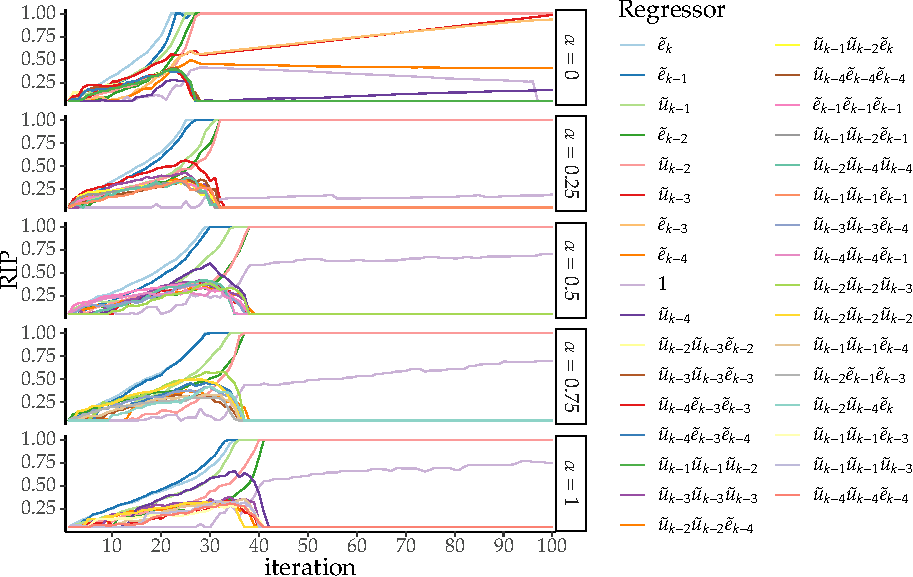
\includegraphics{Figs/Cap5/ex51_rips_evol_SR.tex.pdf}
    \caption{RIPs evolution to different values of parameter $\alpha$ considering data without noise.}
    \label{fig:exp51_ev_rips_a1_SR}
  \end{figure}
Observa-se que ao se aumentar o valor de $\alpha$, regressores que não pertencem ao conjunto de regressores ideais encontram mais dificuldades em serem selecionados, quando comparados com o caso em que nenhuma informação da malha fechada é utilizado (caso com $\alpha=0$1)\footnote{note que o caso em que $\alpha=0$ neste exemplo corresponde ao caso A do Exemplo \ref{ex:sis2aord}.}.

Note que, para esta realização, para $\alpha=0.5$ e $\alpha=1$ o algoritmo foi interrompido por volta das iteração 60 e 90, respectivamente, devido ao critério de parada \eqref{eq:crit.par} ter sido satisfeito. Ressalta-se que isto ocorre para esta realização específica, o mesmo pode não ocorrer para outras realizações, devido ao caráter aleatório do método.
Apesar disso, de forma geral, ao se realizar diversas iterações é possível notar que o comportamento geral da Figura \ref{fig:exp51_ev_rips_a1_SR} prevalece, com maiores escolhas de RIPs espúrios para o caso, em que $\alpha=0$, quando comparado aos demais.

Para analisar o comportamento de uma forma mais geral, foram realizadas 50 realizações (com os mesmos dados de treinamento) para cada valor de $\alpha$. A densidade de probabilidade de convergência dos RIPs para cada valor de $\alpha$, em função do número de iteração é mostrado na Figura \ref{fig:exp51_dens_prob_SR}.
\begin{figure}[htpb]
  \centering
  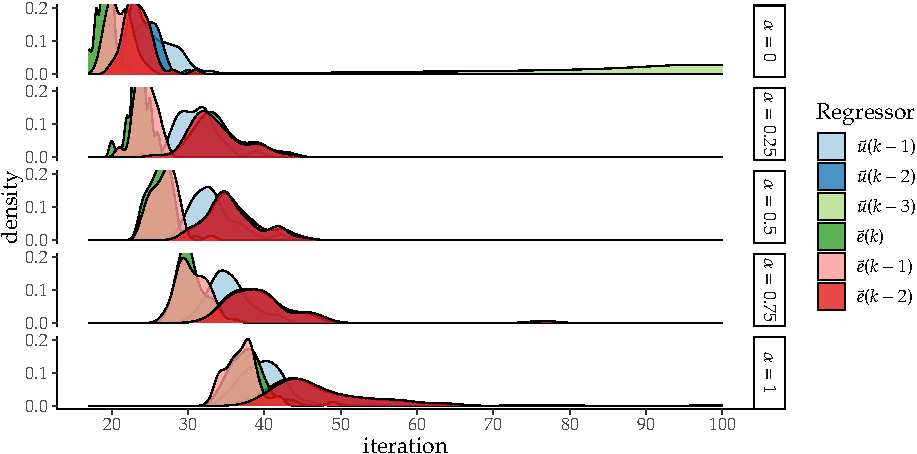
\includegraphics{Figs/Cap5/ex51_iter_con_SEM_ruido.tex.pdf}
  \caption{Probability densities of selection for the regressors selected within 100 iterations considering different values of $\alpha$ for the case without noise.}
  \label{fig:exp51_dens_prob_SR}
\end{figure}
Na figura, fica claro que o método seleciona bem os parâmetros ideais para todos os casos. No caso sem uso de informação do erro de rastreamento, $\alpha=0$, o regressor $\tilde{u}(k-3)$ é escolhido com baixa probabilidade para poucas iterações mas com probabilidade crescente com o aumento das iterações. 

Quando se introduz informações do erro de rastreamento, casos com $\alpha>0$, somente os regressores ideais são selecionados para todos as 50 realizações. Nota-se que o tempo médio geral de de escolha dos regressores aumenta com o aumento do parâmetro $\alpha$. Uma possível explicação é que o índice de desempenho relativo ao erro de rastreamento, $J_r$, muda pouco em relação ao índice relativo ao erro de predição, $J_p$. Uma provável solução pode ser adotar um ganho $K$ maior no cálculo do MSTE (vide equação \ref{eq:Jr}).

As mesmas simulações anteriores são feitas para o caso em que existe ruído de medição (ruído na saída), como no caso B do Exemplo \ref{ex:sis2aord}. A Figura \ref{fig:exp51_ev_rips_a1_CR} mostra a evolução dos RIPs e a Figura \ref{fig:exp51_dens_prob_CR} mostra a densidade de probabilidade de escolha dos regressores em função do número de iterações para cada valor de $\alpha$, considerando esse novo caso.

  \begin{figure}[htpb]
    \centering
    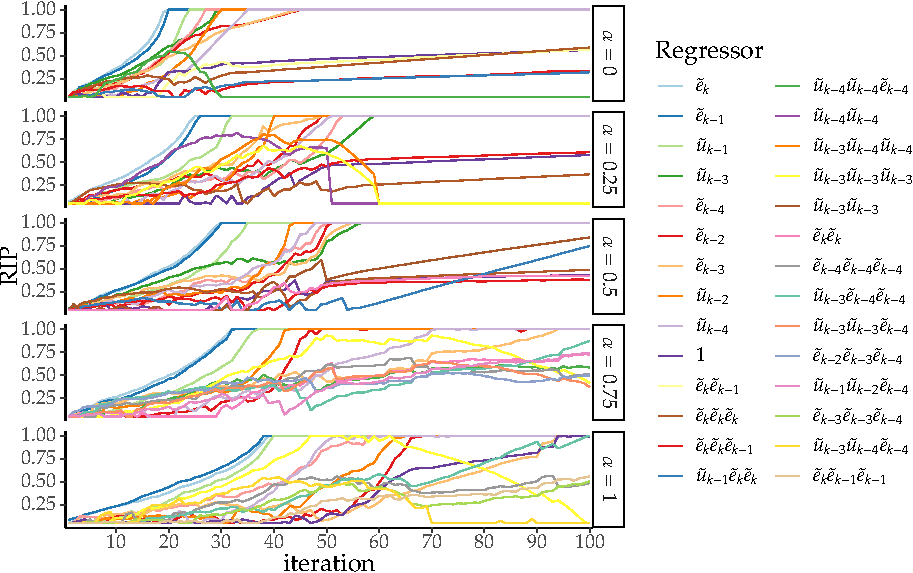
\includegraphics{Figs/Cap5/ex51_rips_evol_CR.tex.pdf}
    \caption{RIPs evolution to different values of parameter $\alpha$ considering data with noise.}
    \label{fig:exp51_ev_rips_a1_CR}
  \end{figure}

    % \footnote{note que são mostrados em cores os RIPs mais relevantes, i.e. aqueles que não convergem para $\mu_{\min}$). Estes outros são mostrados em escala de cinza e não aparecem na legenda por serem muitos (220 regressores). Os repressores ideais são mostrados em linhas mais espessas.}


  \begin{figure}[htpb]
    \centering
    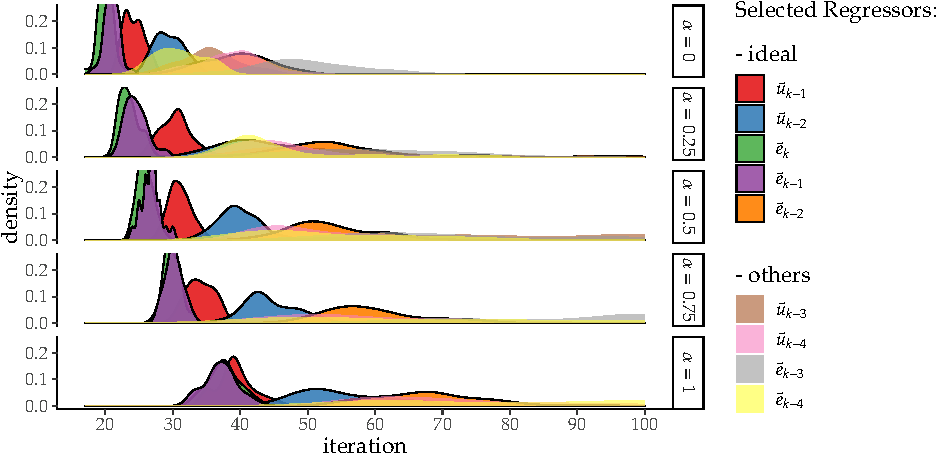
\includegraphics{Figs/Cap5/ex51_iter_con_COM_ruido.tex.pdf}
    \caption{Probability densities of selection for the regressors selected within 100 iterations considering different values of $\alpha$ for the case without noise.}
    \label{fig:exp51_dens_prob_CR}
  \end{figure}

  Observando a Figura \ref{fig:exp51_ev_rips_a1_CR}, observa-se que os seguintes fatores: 1) em todos os casos os regressores ideais foram selecionados. Com o aumento de $\alpha$ os regressores não ideais têm uma menor densidade de probabilidade de serem escolhidos. Isto fica mais evidente comparando-se várias realizações, como mostra a Figura \ref{fig:exp51_ev_rips_a1_CR}. Comparando $\alpha=0$ com $\alpha>0$ nota-se que a probabilidade de ser selecionar regressores não ideiais diminui para menores iterações. Porém para valores maiores de $\alpha$, nota-se um maior tempo de convergência dos regressores. Por exemplo, nota-se uma quantidade maior de regressores que não convergem para o valor mínimo $\mu_{\min}$ para maiores valores de $\alpha$. O problema da polarização pode ser um dos resposponsáveis por este fator.

  % \todo[inline]{    Neste exemplo aplico o ``RaCSS'' ao mesmo sistema de 2a ordem do exemplo anterior, mas agora usando informação do erro de rastreamento no cálculo dos RIPs. \\ Por enquanto estão somente os gráficos, ainda falta análise e algumas tabelas comparativas com ERR.  }

\end{exmp}

